\begin{multicols}{3}[\section{EnOcean}]

\rhead{Alexander Härtel}
\lfoot{19.05.2016}

\newrefsegment

\begin{tabular}{p{2,1 cm}p{2.7 cm}}
\textbf{Steckbrief}& \\
\end{tabular}
\rowcolors{1}{\topicolor!20}{}
\begin{tabular}{p{2,1 cm}p{2.7 cm}}
      Einsatz seit & 2001\\
      Frequenz"-bereich  & \SI{868}{\mega\hertz} für Europa und China, \SI{315}{\mega\hertz} für Asien, \SI{902}{\mega\hertz} für Nordamerika und Kanada, \SI{928}{\mega\hertz} für Japan, \SI{2,4}{\giga\hertz} weltweit offenes Band\\
      Datenrate & \SI{125}{Kbit/s} \\
      Verbreitung & Weltweit\\
      Reichweite & \SI{300}{\metre} im Freifeld \SI{30}{\metre} in Gebäuden\\
      Modulation & FSK in ERP2 und ASK in ERP1\\
      Coding & NRZ\\
      Verschlüsselung & 24-bit Rollingcode und AES mit 128-bit Schlüssel\\
\end{tabular}
\par
\subsection*{Überblick}
\begin{wrapfigure}{r}{0.4\linewidth}
  \vspace{-20pt}
  \begin{center}
  	\hspace{-20pt}
    
\includegraphics[width=1\linewidth]{Kapitel/EnOcean/Grafiken/Eno_alliance_ing_logo_180.jpg}
  \end{center}
  \vspace{-15pt}
\end{wrapfigure}
EnOcean GmbH, ein Spin-off der Siemens AG aus dem Jahr 2001, ist der Entwickler von patentierten batterielosen Funktechnologien. Die EnOcean-Technologie stellt wartungsfreie Funksensorlösungen für den Einsatz in Gebäuden, dem Smart Home und Industrieanlagen sowie für das Internet der Dinge dar.

Die Grundidee für dieses Technologie beruht auf der einfachen Beobachtung, dass überall, wo Sensoren Messwerte erfassen, sich auch ständig der Energiezustand ändert. Schalter werden gedrückt, die Temperatur oder Beleuchtungsstärke schwankt. All diese Vorgänge können gesammelt genug Energie erzeugen, um zum Beispiel Funksignale zu übertragen.

EnOcean bezeichnet den Prozess zur Sammlung dieser Energien \enquote{Energy Harvesting}. Über kinetische Bewegungswandler, Solarzellen sowie Thermowandler ist diese Technologie in der Lage, auf Batterien vollständig zu verzichten. Dieser Aspekt verhilft EnOcean zu ihren wartungsfreien Funklösungen.

\subsection*{Technische Erläuterung}
Zum Senden und Empfangen von Signalen auf in der Regel niedrigen Frequenzbändern oder dem Betrieb von wartungsfreien Sensoren nutzt die EnOcean-Technologie die Energie, die uns tagtäglich umgibt. Der Standard ISO/IEC 14543-3-10 für Funkanwendungen mit einem besonders niedrigen Energieverbrauch wurde unter anderem auf diese Energy Harvesting-Lösungen optimiert. (Quelle enoceanstandard) 

\subsubsection*{Energie durch Bewegung}

\begin{wrapfigure}{r}{0.4\linewidth}
  \vspace{-20pt}
  \begin{center}
  	\hspace{-20pt}
    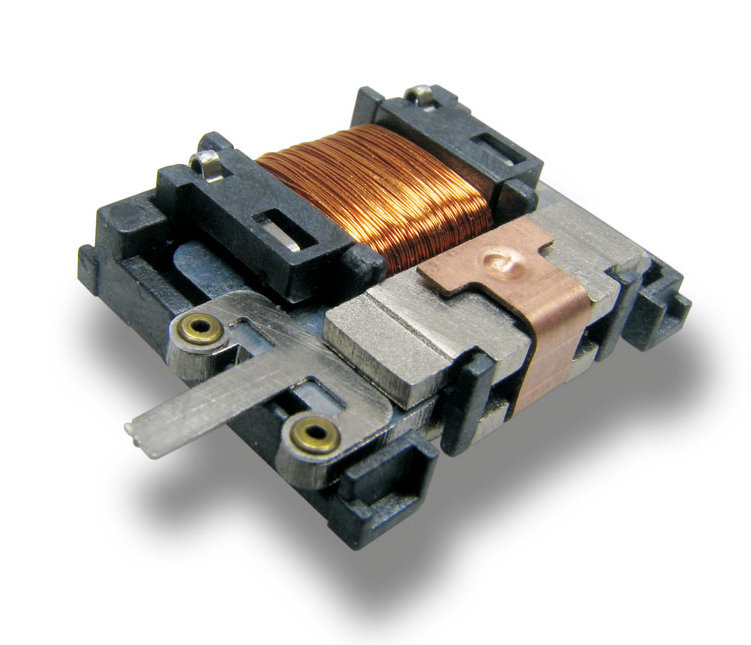
\includegraphics[width=1\linewidth]{Kapitel/EnOcean/Grafiken/EnOceanECO200white.jpg}
    \captionof{figure}{ECO 200~\cite{enocean.2}}
    \label{fig:enocean.eco200}
  \end{center}
  \vspace{-15pt}
\end{wrapfigure}
Der Konverter in Abb.~\ref{fig:enocean.eco200} ist ein ECO 200, der mechanische Energie, wie das Drücken eines Schalters, in elektrische Energie umwandelt. Im Moment befindet er sich im aktiven Einsatz in zahlreichen Produkten. Die Funktionsweise ähnelt dabei einem Dynamo und stellt die Energie sofort zur Verfügung. Mit einem entsprechenden kabel- und batterielosen Modul ist es möglich drei Telegramme pro Operation durchzuführen. Die zur Verfügung gestellte Energie entspricht \SI{120}{\micro\watt\second}.~\cite{enocean.1}

\subsubsection*{Energie durch Licht}
\begin{wrapfigure}{r}{0.4\linewidth}
  \vspace{-20pt}
  \begin{center}
  	\hspace{-10pt}
    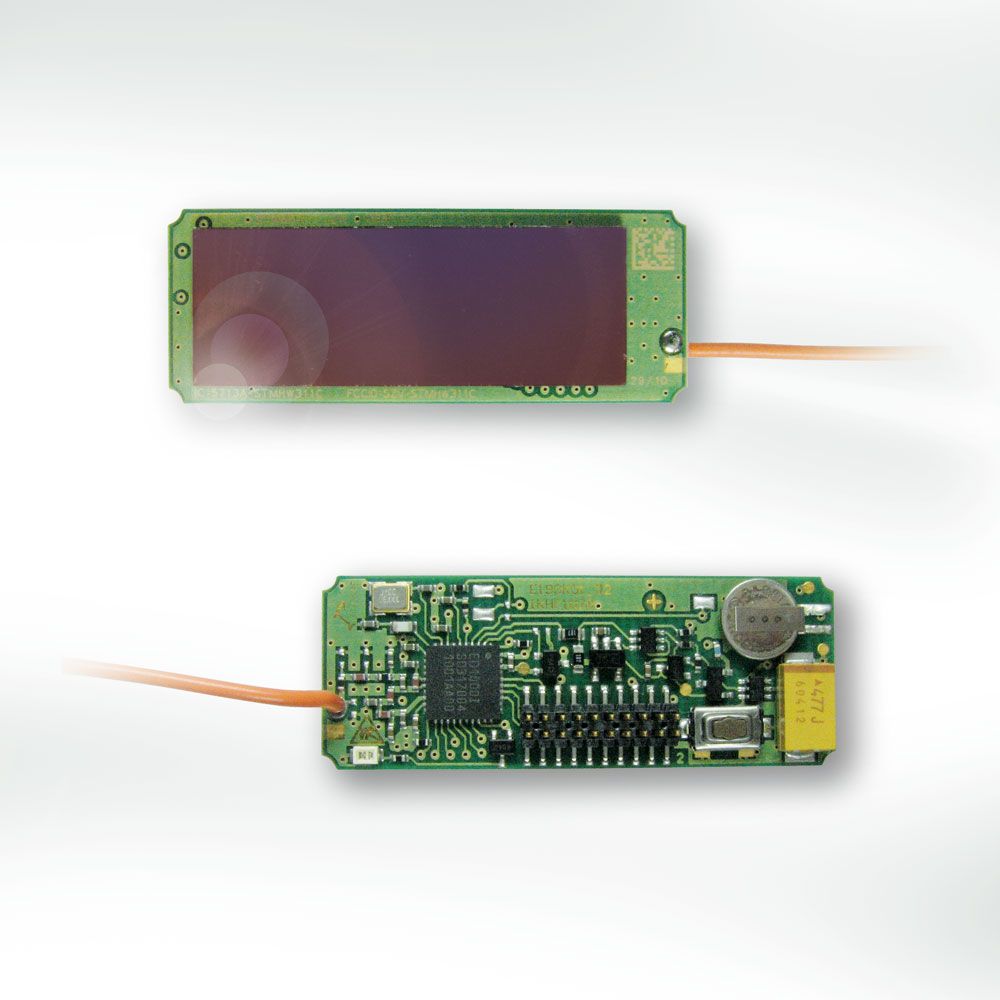
\includegraphics[width=1\linewidth]{Kapitel/EnOcean/Grafiken/EnOcean_STM310_mit_Solarzelle_white.jpg}
    \captionof{figure}{EnOcean STM310 mit Solarzelle~\cite{enocean.3}}
    \label{fig:enocean.stm310}
  \end{center}
  \vspace{-15pt}
\end{wrapfigure}
Zur Umwandlung von Licht in elektrische Energie werden Solarzellen verwendet. Diese Zellen im Miniaturformat, nicht größer als \SI{13}{mm}~x~\SI{35}{mm} wie in Abb.~\ref{fig:enocean.stm310} gezeigt, sind in der Lage allein mit Raumlicht Signale zu senden. Sollte alle \si{15} Minuten ein gemessener Wert übertragen werden, so reichen \si{3,6} Stunden Ladezeit während des Tages bei \si{200} Lux für eine ununterbrochene Operation des Moduls aus.~\cite{enocean.1}

\subsubsection*{Energie durch Temperaturunterschiede}
\begin{wrapfigure}{r}{0.4\linewidth}
  \vspace{-20pt}
  \begin{center}
  	\hspace{-10pt}
    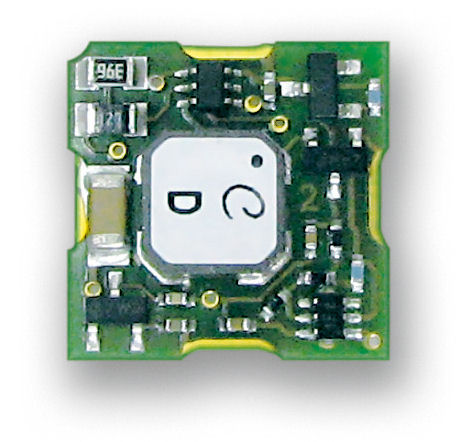
\includegraphics[width=1\linewidth]{Kapitel/EnOcean/Grafiken/EnOceanECT310.jpg}
    \captionof{figure}{EnOcean ECT310~\cite{enocean.5}}
    \label{fig:enocean.ect310}
  \end{center}
  \vspace{-15pt}
\end{wrapfigure}
Zur Gewinnung von Strom durch Änderungen der Umgebungstemperatur werden sogenannte Peltier-Elemente verwendet. Die Funktionsweise basiert auf dem Peltier-Effekt nach Jean Peltier (1785-1845), der bei Stromdurchfluss eine Temperaturdifferenz oder bei Temperaturdifferenz einen Stromfluss erzeugt.~\cite{enocean.4}

Das Peltier-Element in Abb.~\ref{fig:enocean.ect310} liefert bereits bei einer Temperaturdifferenz von ungefähr \SI{2}{K} nutzbare \SI{3}{V} Spannung.~\cite{enocean.1}

\subsubsection*{EnOcean Radio Protocol 2}
Das \textbf{ERP2}~(\textbf{E}nOcean \textbf{R}adio \textbf{P}rotocol 2) wird zur kabellosen Übertragung von Informationen zwischen EnOcean-Sendern und -Empfängern verwendet. Jede Sendung von Daten wird als Telegramm bezeichnet. Dieses Telegramm wird i.d.R. in maximal drei Untertelegramme aufgebrochen. Diese folgen abhängig von der Größe und Art der zu übertragenen Nutzdaten unterschiedlichen strukturellen Definitionen für ihren Aufbau. Des weiteren müssen zusammenhängende Untertelegramme in festen Zeitfenstern übertragen werden.

Da das ERP2 sowie sein Vorgänger ERP1 ohne Kollisionsdetektion arbeiten, müssen höhere Protokolle und Anwendungen damit umgehen können. Optional bietet das ERP2 die Möglichkeit des \textbf{LBT}~(\textbf{L}isten \textbf{b}efore \textbf{t}alk). Bei dieser Funktionalität überprüft das sendende Gerät erst seine Umgebung darauf, ob gerade eine Übertragung von einem Telegramm erfolgt. Sollte dies der Fall sein, so wird für eine zufällige Dauer gewartet. Sollte diese Dauer das Zeitfenster des Untertelegramms überschreiten, so wird dennoch gesendet.~\cite{enocean.6}

\subsubsection*{Sicherheit}
In Anwendungsbereichen, die zusätzliche Datensicherheit benötigen, werden zwei optionale Funktionalitäten zur Verfügung gestellt. Zum einen ein maximal 24-bit langer Rollingcode, der mit jedem Telegramm hochgezählt wird.~\cite{enocean.1}

Rollingcodes finden zum Beispiel bei Garagentoröffnern Anwendung, um den rechtmäßigen Nutzer drahtlos zu authentifizieren. Sie operieren mit einem symmetrischen Schlüssel und einem geeignetem kryptografischen Algorithmus. Vom Sender wird ein sich stets ändernder sogenannter Next-Code übermittlet und vom Empfänger überprüft. Der Empfänger meldet keine Bestätigung zurück.~\cite{enocean.7}

Zum anderen wird der \textbf{AES}~(\textbf{A}dvanced \textbf{E}ncryption \textbf{S}tandard) mit einem 128-bit langen Schlüssel zur Verfügung gestellt.~\cite{enocean.1}

\subsection*{Einsatz}
Die EnOcean-Technologie kann in jedem Bereich zum Einsatz kommen, in dem die Kombination aus drahtlosen, batterielosen und wartungsfreien Geräten bzw. Sensoren sinnvoll ist. Die drei Kernanwendungsgebiete sind Automatisierung/Smart Home, Maschine zu Maschine-Kommunikation und das Internet der Dinge.

So können z.B. Daten über Temperatur-, Licht- oder Gaskonzentrationsveränderungen von Sensoren an eine zentrale Steuerungseinheit geschickt werden, die anschließend diese Daten auswertet und entsprechend handelt. Bei einer Maschinen zu Maschinen-Kommunikation könnte z.B. ein Alarm ausgelöst werden, wenn ein Gasleck durch die Sensoren gemessen wurde.~\cite{enocean.1}

\subsubsection*{Das Internet der Dinge}
Die Sensoren von EnOcean sollen beim Internet der Dinge dort zum Einsatz kommen, wo kabelgebundene oder batteriebetriebene Geräte keine Option darstellen. Hierfür muss unter anderem eine Adressierung über IPv6 möglich sein. IPv6 als Kommunikationsprotokoll ist ursprünglich nicht für Prozesse ausgelegt worden, die mit ihrer verfügbaren Energie haushalten müssen.  

Zur Übertragung von gerade einmal \SI{1}{byte} an gemessen Daten eines Sensors würde bei der Verwendung von IPv6 und UDP ein Overhead von \SI{48}{bytes} für Header entstehen. Zur Umschiffung dieses Overheads wird jedem Sensor ein IP Gateway zugewiesen, dessen Zweck es ist eine Übersetzung zwischen IPv6 und den energieeffizienten EnOcean Sensor Protokollen ISO/IEC 14543-3-1X und IEEE 802.15.4 herzustellen. Letztere Protokolle benötigen nur noch einen Header mit \SI{7}{bytes} Länge.~\cite{enocean.8}

\subsubsection*{Reichweite}
Bei der Reichweite ist zwischen Geräten zu unterscheiden die auf Frequenzbändern unterhalb von \SI{1}{GHz} und solchen die auf \SI{2,4}{GHz} arbeiten. Erstere bieten verlässlichen Transport der Sendungen durch Wände und damit eine Kommunikation bis zu \SI{30}{Meter} innerhalb von Gebäuden und \SI{300}{Meter} auf freiem Feld. Somit sind diese Geräte prädestiniert für die Anwendung in der integrierten Gebäudekontrolle. 

Geräte, die auf dem höheren Frequenzband arbeiten, erreichen innerhalb von Gebäuden eine Reichweite von bis zu \SI{10}{Meter} und auf dem freien Feld von bis zu \SI{100}{Meter}. Sie sind somit eher für Lösungen, die sich auf einen Raum beschränken und keine Penetration von Wänden benötigen, ausgelegt.

Telegramme werden nur gesendet, wenn es notwendig ist. Das heißt, dass z.B. Daten gesammelt wurden oder ein vordefiniertes Zeitfenster %Cut

\end{multicols}
\newpage
\section*{Historische Entwicklung}
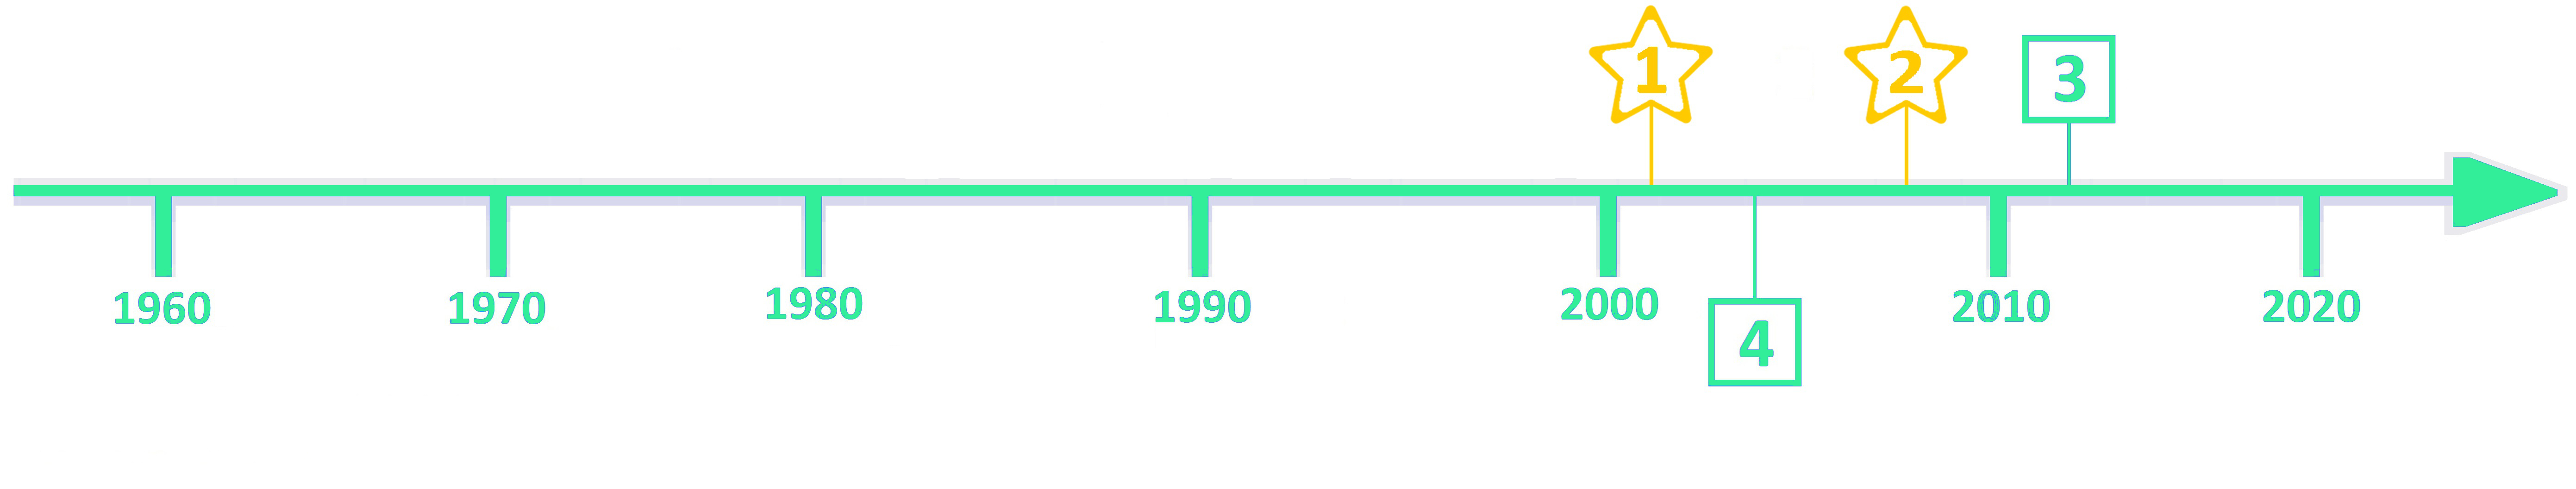
\includegraphics[width=\textwidth]{Kapitel/EnOcean/Grafiken/Zeitstrahl_MitEinfaerben.jpg}
\par
\noindent
\rowcolors{2}{}{\topicolor!20}
\begin{tabular}{p{0.5 cm}p{1.5 cm}p{15.55 cm}}
	Nr. & Datum & Entwicklungsschritte\\
	1 & 2001 & EnOcean wird im Jahr 2001 als Spin-off der Siemens AG gegründet.\\
	2 & 2008 & Die EnOcean Alliance wird gegründet.\\
	3 & 2012 & ISO/IEC 14543-3-10 wird ratifiziert.\\
	4 & 2004 & IEEE 802.15.4 wird ratifiziert.\\
\end{tabular}
\par
\begin{multicols}{3}

abgelaufen ist. Dieses Verhalten verringert Elektrosmog auf den verwendeten Frequenzbändern und erhöht die Anzahl an möglich operierenden Geräten.~\cite{enocean.1}

\subsection*{Anbieter und Gremien}
Die Standardisierung von EnOcean lässt sich in zwei Teile spalten. In die von der \textbf{IEC}~(\textbf{I}nternational \textbf{E}lectrotechnical \textbf{C}ommission) standardisierten Schichten 1 bis 3 und die durch  \textbf{EEP}~(\textbf{E}nOcean \textbf{E}quipment \textbf{P}rofiles) bestimmten darüber liegenden Schichten. 

\begin{Figure}
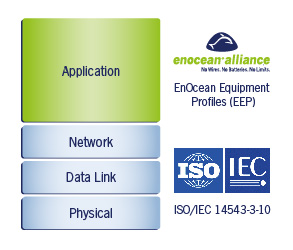
\includegraphics[width=\linewidth]{Kapitel/EnOcean/Grafiken/iso_iec_standard.jpg}
\captionof{figure}{Standardisierung der EnOcean-Technologie~\cite{enocean.9}}
\end{Figure}

\enquote{Die IEC hat mit ISO/IEC 14543-3-10 einen neuen Standard für Funkanwendungen mit einem besonders niedrigen Energieverbrauch ratifiziert. Es ist der erste und einzige Funkstandard, der auch für Energy Harvesting-Lösungen – und damit für die batterielose Funktechnologie von EnOcean – optimiert ist. Zusammen mit den Anwendungsprofilen (EnOcean Equipment Profiles, EEPs) der EnOcean Alliance schafft dieser internationale Standard die Voraussetzungen für eine vollständig interoperable, offene Funktechnologie vergleichbar mit Standards wie Bluetooth oder WiFi.}~\cite{enocean.9}

Die EnOcean Alliance, ein Zusammenschluss aus Unternehmen aus der Gebäudebranche, bestimmten gemeinsam die EPPs. Auf Basis dieser Standards wird gewährleistet, dass Endprodukte unterschiedlicher Anbieter mit einander kompatibel sind. 

\subsection*{Ausblick}
Eine wartungsfreie und skalierbare Kommunikation zwischen Maschinen ist eine der Grundsteine, die benötigt werden um Industire 4.0 umzusetzen. Aber auch die vorschreitende Vernetzung unseres gesamten Alltagslebens mit einander braucht die Funktionalitäten die EnOcean bereits liefern kann. 

Von meiner Perspektive aus wird es besonders Interessant, wenn man diese Technologie mit anderen kombiniert. So wäre es denkbar in Gebieten um z.B. einen Vulkan großflächige Netze aus Sensoren aufzubauen. Senden die Sensoren eines Gebietes dann all ihre Daten an eine Sammelstelle, die die Information schlussendlich den Forschern zur Verfügung stellt, so könnten großflächige Gebiete über mehrere Jahr hinweg beobachtet werden, ohne signifikantes Personal für Wartung abzustellen.

Auch in neuen Häusern oder bei Sanierungen ist der Einbau solcher Technik denkbar. So könnte die Temperatur relativ leicht an unterschiedlichen Stellen im Haus überwacht werden, ohne dort Kabel verlegen zu müssen. Alternativ könnten bestehende Technologien, wie Brandmelder, mit den Energy Harvesting Methoden kombiniert werden, um eine längere Operationsdauer zu gewährleisten.

\printbibliography[segment=16,heading=subbibliography]
\end{multicols}
\newpage
